For two dimensional data, the evaluation covers the following tasks:

\begin{itemize}
 	\item Find hyper-parameters for the LISA Baseline model empirically.
	\item Find the hyper-parameters for the LISA model empirically.
	\item Compares the performance between $K$D-tree, LISA Baseline and LISA models for point query.
	\item Compare the performance between $K$D-tree, LISA Baseline and LISA models for range query.
	\item Compare the performance between $K$D-tree and LISA models for KNN query. KNN Query has not been implemented for LISA Baseline as there is no description of KNN Query for Baseline model in the paper. 
\end{itemize}

\subsection{Dataset}

For two dimensional case, we manually generate three columns of the data:

\begin{itemize}
	\item The first two columns contain the  2 dimensional keys $\boldsymbol{X} \in \mathbb{R}^{2}$, which are independently sampled from a given distribution. %% TOOD: What distributions?
	\item Then we assign the keys into different pages according to a preset parameter $N_{page}$ for page size. Specifically, the first $N_{page}$ keys will be assigned into the first page, the second $N_{page}$ keys will be assigned into the second page and so on so forth. After the assignments, we set the second column $Y$ to be the page index of the corresponding $x$.
\end{itemize}

\subsection{Task 1 : Hyper-parameters Search }
After generating dataset as mentioned in previous section, we sample a smaller subset from it. We repeat our experiments for 3 different sample sizes of 10000, 100000 and 1000000 points. Test data is a copy of training data for all our experiments. For Baseline and Lisa models, final prediction is given by linear search through a range of values (identified as a Cell for Baseline and Shard for LISA model) and mean square error (MSE) is zero as test points are already learned during training. This is where Learned Index models differ from traditional machine learning models where model performance is evaluated on unseen data. 

\subsubsection {Hyper-parameter search for the LISA Baseline implementation}
Baseline model has one hyper parameter: N (Number of cells specifying the number of equal length intervals into which mapped values are divided). As discussed in section, the query search consists of two parts, first is binary search to locate the cell into which the query key is located, followed by sequentially comparison of the query key value with keys in the found cell until a match is found. The time complexity of first search is $log_{2}N_{1}$, where $N_{1}$ is the number of cells. The time complexity of second search is  $ \left \lceil {N_{2} / 2}\right \rceil $, where $N_{2}$ is the number of keys per cell.

\begin{table}[ht]
	\centering
	\begin{tabular}{||p{0.15\textwidth}<{\centering}|p{0.2\textwidth}<{\centering}| p{0.1\textwidth}<{\centering}|p{0.15\textwidth}<{\centering}|p{0.15\textwidth}<{\centering}|p{0.15\textwidth}<{\centering}||}
		\hline
		Training/Test Data Size& Model & No. of cells & Build Time (ms) & Avg Query Time (ms) & Memory Size (KB)\\ [0.5ex] 
		\hline
		\hline
		%10,000& Lisa Baseline & 10 & 11.171 & 4.34261 & 313.77\\
		%\hline
		10,000& LISA Baseline & 100 & 11.252 & 0.71891 & 315\\
		\hline
		10,000& LISA Baseline & 1000 & 13.542 & 0.32806 & 336\\
		\hline
		10,000& LISA Baseline & 10000 &26.831 & 0.19857 & 547\\
		\hline
		\hline
	\end{tabular}
    \caption{Hyper-parameters Search LISA Baseline Model: Training Size:10,000 Points}
    \label{small_lognormal_lisa_baseline_10000}
\end{table}

\begin{table}[ht]
	\centering
	\begin{tabular}{||p{0.15\textwidth}<{\centering}|p{0.2\textwidth}<{\centering}| p{0.1\textwidth}<{\centering}|p{0.15\textwidth}<{\centering}|p{0.15\textwidth}<{\centering}|p{0.15\textwidth}<{\centering}||}
		\hline
		Training/Test Data Size & Model & No. of cells & Build Time (ms) & Avg Query Time (ms) & Memory Size (KB)\\ [0.5ex] 
		\hline
		\hline
		%100,000& Lisa Baseline & 10 & 109.287 & 46.7233 & 3126.2\\
		%\hline
		%100,000& Lisa Baseline & 100 & 111.596 & 4.8086 & 3128.3\\
		
		100,000& LISA Baseline & 1000 & 111.978 & 0.7271 & 3149\\
		\hline
		100,000& LISA Baseline & 10000 & 128.496 & 0.3301 & 3360\\
		\hline
		100,000& LISA Baseline & 100000 & 272.933 & 0.2381 & 5469\\
		\hline
		\hline
	\end{tabular}
   \caption{Hyper-parameters Search LISA Baseline Model: Training Size:100,000 Points}
    \label{small_lognormal_lisa_baseline_100000}
\end{table}

\textbf{Conclusion} As shown in tables \ref{small_lognormal_lisa_baseline_10000}, \ref{small_lognormal_lisa_baseline_100000} and \ref{small_lognormal_lisa_baseline_1000000}, following conclusions can be drawn:
\begin{enumerate}
	\item Build time : Build time increases with increase in value of N, as metadata for additional cells needs to be calculated. 
	\item Average Query Time :  Average Query Time decreases with increase in value of N as number of keys per cell decreases.
	\item Memory Size :  Memory requirements of the model increases with increase in value of N, as metadata for additional cells needs to be stored. Increase  in memory size is not significant with increase in number of cells as we maintain only two values per cell, mapped value of first key in the cell and mapped value of last key in the cell.
\end{enumerate}

\begin{table}[ht]
	\centering
	\begin{tabular}{||p{0.15\textwidth}<{\centering}|p{0.2\textwidth}<{\centering}| p{0.1\textwidth}<{\centering}|p{0.15\textwidth}<{\centering}|p{0.15\textwidth}<{\centering}|p{0.15\textwidth}<{\centering}||}
		\hline
		Training/Test Data Size& Model & No. of cells & Build Time(ms) & Avg Query Time(ms) & Memory Size(KB)\\ [0.5ex] 
		\hline
		\hline
		%1,000,000& Lisa Baseline & 10 & 1094.99 & 347.561 & 31251.3\\
		%\hline
		%1,000,000& Lisa Baseline & 100 &1099.68 &40.145 & 31253.4\\
		%\hline
		1,000,000& LISA Baseline & 1000 & 1104.65 & 4.473 & 31274.5\\
		\hline
		1,000,000& LISA Baseline & 10000 & 1143.73 & 0.669 & 31485.4\\
		\hline
		1,000,000& LISA Baseline & 100000 & 1273.56 & 0.294 & 33594.8\\
		\hline
		1,000,000& LISA Baseline & 1000000 & 2717.65 & 0.243 & 54688.5\\
		\hline
		\hline
	\end{tabular}
    
	\caption{Hyper-parameters Search LISA Baseline Model: Training Size:1,000,000 Points}
	\label{small_lognormal_lisa_baseline_1000000}
\end{table}



\subsubsection {Hyper-parameter search for the LISA implementation}
For LISA model, we have 3 hyper parameters:
\begin{enumerate}
	\item $G$ : The size of the grid cell. Number of grid cells into which the key space is divided. In our implementation, we use a square grid cell, and total number of cells is given by $G$ $\times G$.
	\item $N$ : Number of equal length intervals into which mapped value range is divided. During our experiments, we found that shard prediction algorithm gives best performance if mapped interval boundaries are aligned to grid cell boundaries. That's why this parameter is initialized to $N$=$G$ $\times G$   
	\item $S$ : Number of shards to learn per mapped interval. 
\end{enumerate}

\textbf{Conclusion} Experiments results shown in tables \ref{small_lognormal_lisa_10000}, \ref{small_lognormal_lisa_100000} and \ref{small_lognormal_lisa_1000000} are consistent across all 3 training sizes and have following interpretation. 
\begin{enumerate}
    \item Average query time decreases and memory size increases with increase in values of $G$ and $S$. 
	\item For a particular value of $G$, average query time decreases and memory size increases with increase in value of S.
	\item We need to choose S such that there are at least 35 keys per shard. We see mse errors if number of keys per shard are less than 35 for following reasons. 
	\begin{enumerate}
	    \item Total number of keys are first divided equally among grid cells, and for each cell, we divide the keys falling in that cell equally among number of shards.
	    \item For point query search, we first predict a shard and then sequentially compare the query point key values with all the keys in the predicted shard until a match is found
		\item For query points near the shard boundaries, there can be a mismatch in groundtruth shardId and predicted shardId.If the query point is not found in the predicted shard, we continue our search in adjacent left and right shards in an empirically found range.
	\end{enumerate}
	
	During test experiments we found that if shard size is less than 35 keys, then sometimes shard prediction error can be greater than 1 and point query search can fail resulting in mse errors.  
\end{enumerate}

\begin{table}
	\centering
	\begin{tabular}{||p{0.14\textwidth}<{\centering}|p{0.08\textwidth}<{\centering}|p{0.15\textwidth}<{\centering}| p{0.07\textwidth}<{\centering}|p{0.1\textwidth}<{\centering}|p{0.125\textwidth}<{\centering}|p{0.125\textwidth}<{\centering}|p{0.07\textwidth}<{\centering}||}
		\hline
		Training/Test Data Size& Model & G & S& Build Time(s) & Avg Query Time(ms) & Memory Size(KB) &mse\\ [0.5ex] 
		\hline
		\hline
		10,000& LISA& 4*4=16 & 5& 4.335& 1.13135 & 324.72&0\\
		\hline
		10,000& LISA& 4*4=16 & 10& 3.370& 0.96036 & 329.07&0\\
		\hline
		10,000& LISA& 4*4=16 & 20&1.127& 0.86184 & 337.85&0\\
		\hline
		10,000& LISA& 4*4=16 & 30&3.478& 0.74339 & 346.63&5729\\
		\hline
	    \hline
	\end{tabular}

    \caption{Hyper-parameters Search LISA Model: Training Size:10,000 Points. \\
    a) For the last row, Numbers of keys= 10000 \\
    b) Keys per cell= $10000 \setminus (4\times4) = 625$\\
    c) Keys per shard = $625\setminus30=20$ keys per shard, resulting in mse errors}
	\label{small_lognormal_lisa_10000}
\end{table}

\begin{table}
	\centering
	\begin{tabular}{||p{0.14\textwidth}<{\centering}|p{0.08\textwidth}<{\centering}|p{0.15\textwidth}<{\centering}| p{0.07\textwidth}<{\centering}|p{0.1\textwidth}<{\centering}|p{0.125\textwidth}<{\centering}|p{0.125\textwidth}<{\centering}|p{0.08\textwidth}<{\centering}||}
		\hline
		Training/Test Data Size& Model & GridCellSize & No of Shards & Build Time(s) & Avg Query Time(ms) & Memory Size(KB)&mse\\ [0.5ex] 
		\hline
		\hline
	    %100,000& Lisa& 4*4=16 & 5& 45.846& 5.93345 & 3137.2&0\\
		%\hline
		%100,000& Lisa& 4*4=16 & 10& 42.398& 3.29308 & 3141.6&0\\
		%\hline
		100,000& LISA& 4*4=16 & 20& 59.036&1.52851 & 3150.3&0\\
		\hline
		100,000& LISA& 4*4=16 & 50& 122.64& 1.51173 & 3176.6&0\\
		\hline
		100,000& Lisa& 4*4=16 & 100& 30.211& 1.44084 & 3220.3&0\\
		\hline
		100,000& LISA& 4*4=16 & 150& 142.13&1.15491 & 3264.1&297234\\
		%\hline
		%100,000& Lisa& 6*6=36 & 20&33.637&1.59742 & 3178.9&0\\
		\hline
		100,000& Lisa& 6*6=36 & 50& 66.375& 1.55903 & 3238.1&0\\
		\hline
		100,000& LISA& 6*6=36 & 75& 72.491& 1.43043 & 3287.2&0\\
		\hline
		100,000& Lisa& 6*6=36 & 100& 60.929& 1.64881 & 3336.4&5.6e+07\\
		\hline
		100,000& LISA& 8*8=64 & 20& 35.638& 1.54029 & 3218.7&0\\
		\hline
		100,000& LISA& 8*8=64 & 50& 45.014& 1.52117 & 3323.6&0\\
		\hline
		\hline
	\end{tabular}
    \caption{Hyper-parameters Search LISA Model: Training Size:100,000 Points}
	\label{small_lognormal_lisa_100000}
\end{table}

\begin{table}
	\centering
\centering
	\begin{tabular}{||p{0.14\textwidth}<{\centering}|p{0.08\textwidth}<{\centering}|p{0.15\textwidth}<{\centering}| p{0.07\textwidth}<{\centering}|p{0.1\textwidth}<{\centering}|p{0.125\textwidth}<{\centering}|p{0.125\textwidth}<{\centering}|p{0.08\textwidth}<{\centering}||}
		\hline
		Training/Test Data Size& Model & GridCellSize & No of Shards& Build Time(s) & Avg Query Time(ms) & Memory Size(KB)&mse\\ [0.5ex] 
		\hline
		\hline
	 	%1,000,000&Lisa& 10*10=100 & 5& 122.64& 1.51173 & 3176.6&0\\
		%\hline
		%1,000,000& Lisa& 10*10=100 & 10& 30.211& 1.44518 & 3220.3&0\\
		%\hline
		%1,000,000& Lisa& 10*10=100 & 20& 24.428&3.19491 & 3149.4&0\\
		%\hline
		1,000,000& LISA& 10*10=100 & 50&743.29&1.77751 & 31558.9&0\\
		\hline
		1,000,000& Lisa& 10*10=100 & 100& 1077.89& 1.63397 & 31832.3&0\\
		\hline
		1,000,000& LISA& 20*20=400 & 25& 365.49& 2.53317 & 31930.8&0\\
		\hline
		1,000,000& LISA& 20*20=400 & 50& 609.32& 1.44526 & 32477.6&0\\
		\hline
		1,000,000& LISA& 25*25=625 & 25& 240.22& 1.56227& 32779.8&0\\
		\hline
		1,000,000& LISA& 30*30=900 & 25& 205.18& 1.79839 & 33010.3&0\\
		\hline
		\hline
	\end{tabular}
    \caption{Hyper-parameters Search LISA Model: Training Size:1,000,000 Points}
	\label{small_lognormal_lisa_1000000}
\end{table}

\subsection{Point Query Comparison for $K$D-Tree, LISA-Baseline and LISA Models }
Table \ref{Point_Query_Comparision} shows the performance evaluation for $K$D-Tree, LISA-Baseline and LISA Models for different training data sizes. For a given training set, we perform point query evaluation for every point in the dataset and take the average. As shown in the Fig. \ref{fig:Point_Query_Comparision}, LISA outperforms $K$D-tree in terms of average query time and memory requirements, however its build time is significantly higher than $K$D-Tree 

\begin{table}
	\centering
\centering
	\begin{tabular}{||p{0.18\textwidth}<{\centering}|p{0.15\textwidth}<{\centering}|p{0.15\textwidth}<{\centering}|p{0.15\textwidth}<{\centering}|p{0.15\textwidth}<{\centering}|p{0.05\textwidth}<{\centering}||}
		\hline
		Training/Test Data Size& Model & Build Time(s) & Avg Query Time(ms) & Memory Size(KB)&mse\\ [0.5ex] 
		\hline
		\hline
	 	10,000& KD-Tree & 0.023 & 4.363 & 2890 & 0\\
	 	\hline
	 	10,000& Baseline & 0.026 & 0.198 & 547&0\\
	 	\hline
	 	10,000& LISA & 1.127&0.861 & 337&0\\
		\hline
	 	100,000& KD-Tree & 0.340 & 6.176 & 28906 &0\\
	 	\hline
	 	100,000& Baseline & 0.324 & 0.241 & 5469&0\\
	 	\hline
	 	100,000& LISA& 22.491& 1.43 & 3169&0\\
		\hline
	 	1,000,000& KD-Tree& 4.124 & 9.254 & 289062 &0\\
	 	\hline
	 	1,000,000& Baseline& 2.718 & 0.343 & 54688&0\\
	 	\hline
	 	1,000,000& LISA& 445.324&1.445 & 32477&0\\
	 	
	 	%\hline
	 	%10,000,000& KD-Tree& 77.924 & 10.254 & 2421880 &0\\
	 	%\hline
	 	%10,000,000& Baseline& 13.118 & 3.873 & 312736&0\\
	 	%\hline
	 	%10,000,000& LISA& 445.324&1.445 & 32477&0\\
		\hline
		\hline
	\end{tabular}
	\caption{Point Query experimental results for KDTree, Baseline and LISA models}
	\label{Point_Query_Comparision}
\end{table}

\begin{figure*}[t]
    \centering
    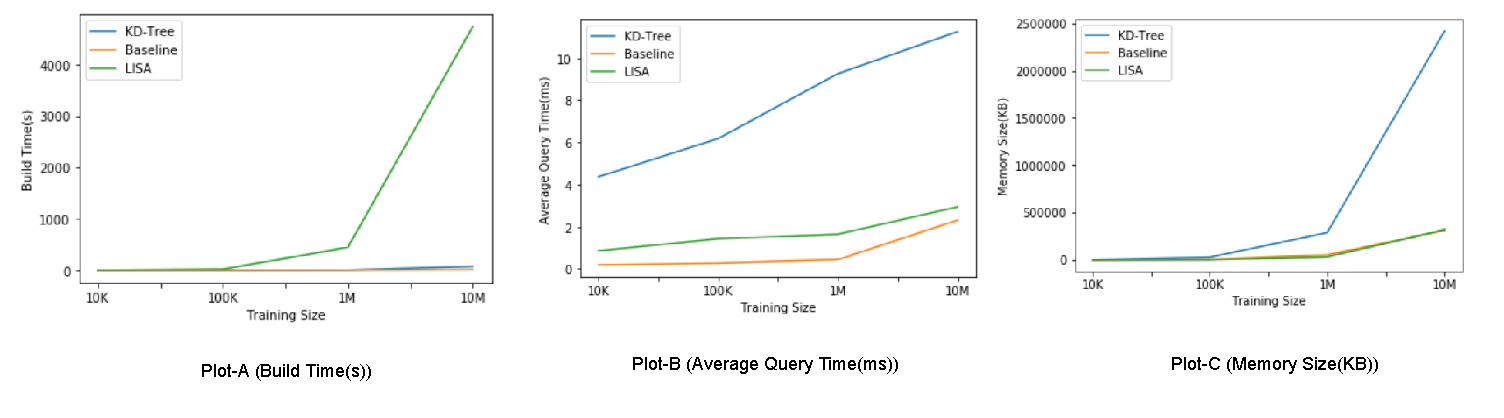
\includegraphics[width=1.1\textwidth]{graphs/evaluation/PointQueryPlot.pdf}
    \caption{Point Query experimental results for $K$D-Tree, Baseline and LISA models\\
    LISA outperforms $K$D-Tree in terms of average query time and memory requirements, however its build time is significantly higher than $K$D-Tree }
    \label{fig:Point_Query_Comparision}
\end{figure*}
\subsubsection {Range Query Experiments}
Table \ref{Range_Query_Experimental_Results} shows evaluation results for LISA,Baseline and $K$D-tree models for range sizes of 10, 100, 1000 for different training sizes. For a given range query size, we perform 20 trials and take the average. For each trial, we sample a random point from the test set and find the range from sampled point to the range query size. Average query time for each range is further divided by the range size to compare the query time across various ranges. 

\begin{figure*}
    \centering
    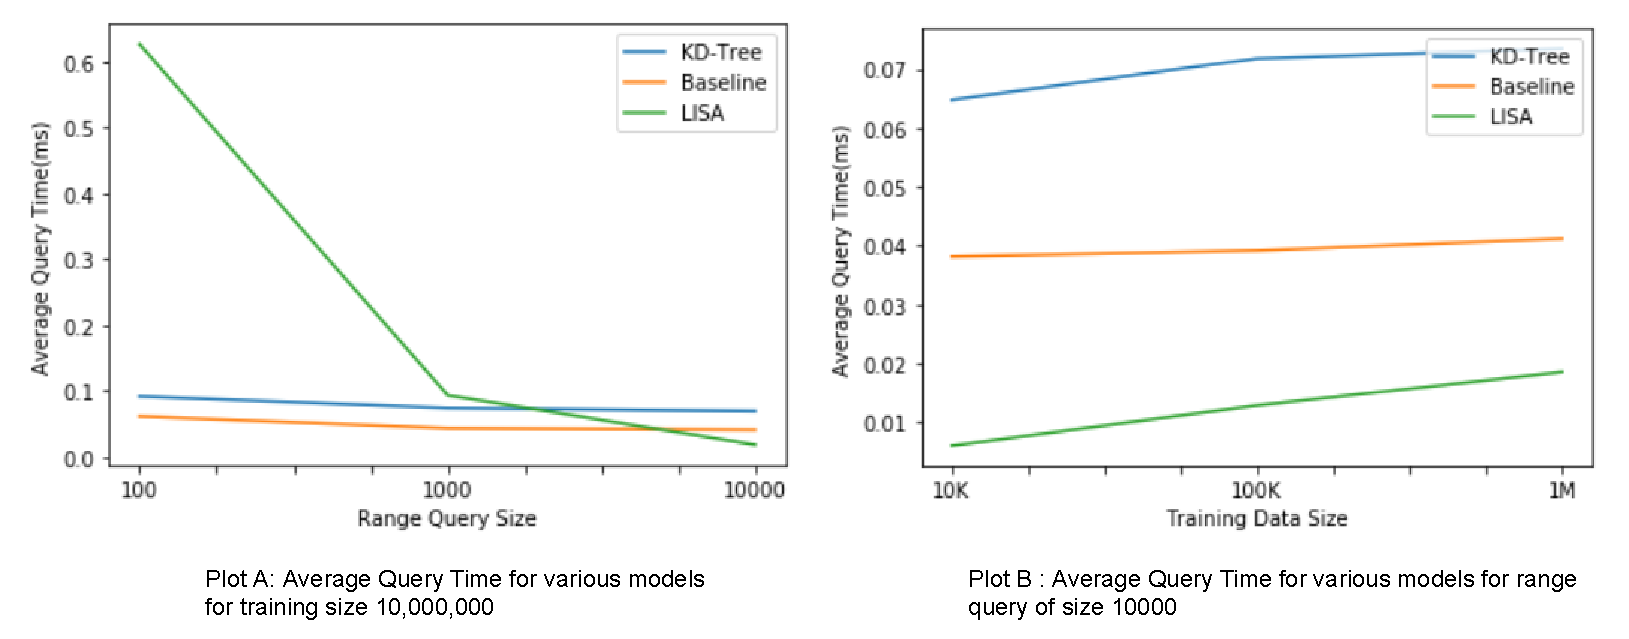
\includegraphics[width=1.1\textwidth]{graphs/evaluation/RangeQueryPlot.pdf}
    \caption{Range Query experimental results for $K$D-Tree, Baseline and LISA models\\
    a) Plot A shows average query time for a fixed training size of 1M points. LISA outperforms $K$D-Tree for larger range queries. \\
     b) Plot B shows average query time for a fixed range query of size 10000 for various training sizes. Lisa outperforms $K$D-Tree for all training data sizes for range queries of size 10000 }
    \label{fig:Range_Query_Comparision}
\end{figure*}

\begin{table}
	\centering
\centering
	\begin{tabular}{||p{0.15\textwidth}<{\centering}|p{0.15\textwidth}<{\centering}|p{0.22\textwidth}<{\centering}|p{0.25\textwidth}<{\centering}|p{0.20\textwidth}<{\centering}||}
		\hline
		Training/Test Data Size& Range Query Size & Avg Query Time(ms)($K$D-tree) & Avg Query Time(ms)(Baseline)&Avg Query Time(ms)(LISA)\\ [0.5ex] 
		\hline
		\hline
	 	10,000& 10& 0.2062 & 0.1113& 0.8204 \\
	 	\hline
	 	10,000& 100& 0.0839 & 0.0451& 0.1201 \\
	 	\hline
	 	10,000& 1000& 0.0701 & 0.0399& 0.0294 \\
 	 	\hline
 	 	10,000& 10000& 0.0648&0.0382&0.0061 \\
	 	\hline
	 	100,000& 10& 0.2123 & 0.1298&2.8961 \\
	 	\hline
	 	100,000& 100& 0.0912 & 0.0505&0.2792 \\
	 	\hline
	 	100,000& 1000& 0.0726 & 0.0428&  0.0563 \\
 	 	\hline
 	 	100,000& 10000&0.0718& 0.0392& 0.0129 \\
	 	\hline
	    1,000,000& 10& 0.2238 & 0.2661& 3.5181 \\
	 	\hline
	 	1,000,000& 100& 0.0922 & 0.0617&0.6263 \\
	 	\hline
	 	1,000,000& 1000& 0.0744 & 0.0437 &0.0939 \\
	 	\hline
	 	1,000,000& 10000& 0.0735 & 0.0412 &0.0186 \\
	 	%\hline
	 	%10,000,000& 10& 0.2285 & 0.037188 &12.891 \\
	 	%\hline
	 	%10,000,000& 100& 0.0779 & 0.037188 &0.1611 \\
	 	%\hline
	 	%10,000,000& 1000& 0.0740 &  0.037188 &0.0353 \\
	 	
	 	%\hline
	 	%10,000,000& 10000& 0.0773 &  0.037188 &0.0 \\
	 
		\hline
		\hline
	\end{tabular}
	\caption{Range Query experimental results for $K$D-tree, Baseline and LISA models}
	\label{Range_Query_Experimental_Results}

\end{table}



\subsubsection {$\boldsymbol{K}$NN Query Experiments}
Table \ref{KNN_Query_Experimental_Results} shows evaluation results for LISA and $K$D-tree models for $\boldsymbol{K}$NN Queries for various value of K and training sizes. For a given $\boldsymbol{K}$ value, we perform 20 trials and take the average of query time. For each trial, we sample a random point from the test set and find K neighbours around that point. Average query Time is further divided by $\boldsymbol{K}$ to compare the Query time across various values of $\boldsymbol{K}$.

\begin{table}
	\centering
\centering
	\begin{tabular}{||p{0.15\textwidth}<{\centering}|p{0.25\textwidth}<{\centering}|p{0.25\textwidth}<{\centering}|p{0.25\textwidth}<{\centering}||}
		\hline
		Training/Test Data Size& K & Avg Query Time(ms)($K$D-tree) & Avg Query Time(ms)(LISA)\\ [0.5ex] 
		\hline
		\hline
	 	10,000& 3& 1.4069 &0.1927 \\
	 	\hline
	 	10,000& 5& 0.8753 &0.1181\\
	 	\hline
	 	10,000& 7& 0.6333 &0.0811 \\
	 	\hline
	 	10,000 & 10& 0.4368 &0.0549 \\
	 	\hline
	 	100,000 & 3& 2.0325 &0.3406 \\
	 	\hline
	 	100,000 & 5& 1.2004 &0.2884 \\
	 	\hline
	 	100,000 & 7& 0.8812 &0.2158 \\
	 	\hline
	 	100,000 & 10&  0.6618 &0.1577 \\
	 	\hline
	    1,000,000 & 3& 2.7865 & 0.4272 \\
	 	\hline
	 	1,000,000 & 5& 1.7072 &0.6466 \\
	 	\hline
	 	1,000,000 & 7& 1.3255 &0.6024 \\
	 	\hline
	 	1,000,000 & 10& 0.9172 &0.3291 \\
		\hline
		\hline
	\end{tabular}
	\caption{KNN Query experimental results for $K$D-tree and LISA model}
	\label{KNN_Query_Experimental_Results}

\end{table}
